% ============================================================================================================
% Chapter 6 -- Vortices in Two Dimensions: the Kosterlitz--Thouless Flow
% Every number quoted from a computation is a macro \cn... defined in the block below; the block is generated from
% figures/ch06_numbers.json by figures/ch06_inject_macros.py (do not edit it by hand).
% ============================================================================================================
% BEGIN ch06 numbers
\newcommand{\cnBackCvodeU}{0.21}
\newcommand{\cnBackCvodeY}{0.23}
\newcommand{\cnBackL}{-0.663}
\newcommand{\cnBackLb}{-0.226}
\newcommand{\cnBackU}{0.9}
\newcommand{\cnBackY}{0.041}
\newcommand{\cnBoundMed}{0.55}
\newcommand{\cnCdiff}{4.351}
\newcommand{\cnCdiffA}{4.368}
\newcommand{\cnCdiffB}{4.349}
\newcommand{\cnCommitShort}{\texttt{5db8041}}
\newcommand{\cnCritA}{1.78}
\newcommand{\cnCritB}{1.96}
\newcommand{\cnCritC}{1.9993}
\newcommand{\cnCritDevB}{0.0074}
\newcommand{\cnCritDevC}{5\times10^{-5}}
\newcommand{\cnCritDrift}{1.9\times10^{-13}}
\newcommand{\cnCtlHi}{0.25}
\newcommand{\cnCtlLo}{9.5\times10^{-4}}
\newcommand{\cnCtlRatioHi}{1.3\times10^{10}}
\newcommand{\cnCtlRatioLo}{5\times10^{7}}
\newcommand{\cnDfourHi}{0.95}
\newcommand{\cnDfourLo}{0.79}
\newcommand{\cnDhiHundred}{56}
\newcommand{\cnDhiSixtyfour}{28}
\newcommand{\cnDloHundred}{12}
\newcommand{\cnDloSixtyfour}{10}
\newcommand{\cnDriftAdamsA}{2.3\times10^{-5}}
\newcommand{\cnDriftAdamsD}{1.9\times10^{-11}}
\newcommand{\cnDriftBdfA}{6.0\times10^{-6}}
\newcommand{\cnDriftBdfD}{6.3\times10^{-10}}
\newcommand{\cnEhighHundred}{32.2}
\newcommand{\cnEhighSixtyfour}{27.9}
\newcommand{\cnElowHundred}{20.8}
\newcommand{\cnElowSixtyfour}{19.8}
\newcommand{\cnEscN}{9}
\newcommand{\cnEscRatioHi}{0.98}
\newcommand{\cnEscRatioLo}{0.74}
\newcommand{\cnEscRelErr}{2.6\times10^{-11}}
\newcommand{\cnEssOffset}{3.07}
\newcommand{\cnEssRatioA}{0.59}
\newcommand{\cnEssRatioB}{0.95}
\newcommand{\cnEssRatioC}{0.998}
\newcommand{\cnEssRel}{5.6\times10^{-6}}
\newcommand{\cnEtaCrossSixtyfour}{0.307}
\newcommand{\cnEtaKhi}{1.22}
\newcommand{\cnEtaKhiThirtytwo}{1.27}
\newcommand{\cnEtaKlo}{1.12}
\newcommand{\cnEtaKloThirtytwo}{1.14}
\newcommand{\cnFc}{1.723}
\newcommand{\cnJump}{3.49}
\newcommand{\cnKRcv}{0.715}
\newcommand{\cnKRgrid}{0.654}
\newcommand{\cnKseedA}{4.63}
\newcommand{\cnKseedB}{3.56}
\newcommand{\cnKzeroC}{0.7734}
\newcommand{\cnLnThreeEighty}{5.94}
\newcommand{\cnMaxHundred}{0.064}
\newcommand{\cnMaxSixtyfour}{0.071}
\newcommand{\cnMaxUstarErr}{3.3\times10^{-4}}
\newcommand{\cnNbelow}{18}
\newcommand{\cnNbetween}{9}
\newcommand{\cnNbetweenTrapped}{9}
\newcommand{\cnNconfigs}{33}
\newcommand{\cnNhyp}{20}
\newcommand{\cnNlambda}{7.65}
\newcommand{\cnNlambdaExcess}{29}
\newcommand{\cnNsOverNCross}{0.52}
\newcommand{\cnNslGrid}{4.11}
\newcommand{\cnNtraj}{43}
\newcommand{\cnNvMid}{126}
\newcommand{\cnPairHi}{1.6}
\newcommand{\cnPairLo}{0.6}
\newcommand{\cnPairMid}{1.1}
\newcommand{\cnPfourNew}{354}
\newcommand{\cnPfourOld}{353\,469}
\newcommand{\cnPoneNew}{511}
\newcommand{\cnPoneNewErr}{2.0\times10^{-7}}
\newcommand{\cnPoneOld}{237\,022}
\newcommand{\cnPoneOldErr}{6.4\times10^{-4}}
\newcommand{\cnPremiseOk}{32}
\newcommand{\cnPthreeNew}{64}
\newcommand{\cnPthreeOld}{12\,898}
\newcommand{\cnRemMed}{0.12}
\newcommand{\cnRemMedPct}{12}
\newcommand{\cnRmsHundred}{0.033}
\newcommand{\cnRmsSixtyfour}{0.043}
\newcommand{\cnShaShort}{\texttt{0bdb1b4a504f}}
\newcommand{\cnShiftA}{6.1\%}
\newcommand{\cnShiftB}{3.8\%}
\newcommand{\cnShiftC}{2.6\%}
\newcommand{\cnShiftD}{1.4\%}
\newcommand{\cnShiftField}{9}
\newcommand{\cnShiftToy}{1}
\newcommand{\cnSlopeCrossSixtyfour}{32}
\newcommand{\cnSlopeCrossThirtytwo}{13}
\newcommand{\cnSlopeHundred}{1.04}
\newcommand{\cnSlopeSixtyfour}{1.07}
\newcommand{\cnTauHiFields}{1.00}
\newcommand{\cnTauHiRuns}{0.11}
\newcommand{\cnTauLoFields}{0.04}
\newcommand{\cnTauLoRuns}{0.04}
\newcommand{\cnTbktSeedHi}{0.836}
\newcommand{\cnTbktSeedHiThirtytwo}{0.912}
\newcommand{\cnTbktSeedLo}{0.809}
\newcommand{\cnTbktSeedLoThirtytwo}{0.877}
\newcommand{\cnTbktSixtyfour}{0.821}
\newcommand{\cnTbktThirtytwo}{0.893}
\newcommand{\cnTwoPiLnTwo}{4.355}
\newcommand{\cnUstarErrTypical}{2.1\times10^{-9}}
\newcommand{\cnUzeroC}{1.293}
% END ch06 numbers
\chapter{Vortices in Two Dimensions: the Kosterlitz--Thouless Flow}\label{ch06}

\section{A jump fixed by constants}\label{ch06:intro}

A thin film of liquid helium-4 is adsorbed on a substrate that is made to oscillate, and the film is cooled. Bishop and Reppy~\cite{BishopReppy1978} read two things from the
response of the oscillating substrate: the superfluid mass of the film and the dissipation. Both change near a temperature $T_c$, and the way they change was compared with a
theory five years old. Kosterlitz and Thouless~\cite{KosterlitzThouless1973} had proposed that a two-dimensional superfluid does not lose its superfluidity gradually, as a
bulk superfluid does, but abruptly, through the unbinding of pairs of vortices; Nelson and Kosterlitz~\cite{NelsonKosterlitz1977} had drawn the consequence that the superfluid
density must \emph{jump} at the transition, by an amount fixed by constants of nature. The abstract of the letter reports that the superfluid mass and the dissipation, analysed
with the dynamic theory of Ambegaokar, Halperin, Nelson and Siggia~\cite{AHNS1980}, support the Kosterlitz--Thouless picture, and that the predicted jump,
$\rho_s(T_c^-)=8\pi k_B\,(m/h)^2\,T_c$, is in good agreement with estimates from the experiment.

Look at the right-hand side. Apart from the transition temperature, everything in it is a constant of nature: Boltzmann's constant, Planck's constant, and the mass $m$ of a helium
atom. With $m=4.002\,603\,254\,13$ atomic mass units (the NIST value for $^4$He) and the CODATA values of the constants shipped with SciPy, the number is
\[
  \frac{\rho_s(T_c^-)}{T_c}=8\pi k_B\Big(\frac{m}{h}\Big)^{2}=\cnJump\times10^{-9}\ \mathrm{g\,cm^{-2}\,K^{-1}},
\]
computed by \texttt{figures/ch06\_constants.py}. Theory says that the superfluid areal mass density just below the transition is this number times the temperature at which the
transition happens, whatever the substrate, the thickness of the film, or the strength of the interatomic forces; the last sentence of the abstract is a comparison of that number with the experiment. In the units of this book, with the
thermal wavelength $\lambda_T^2=2\pi\hbar^2/(mk_BT)$ and the superfluid number density $n_s=\rho_s/m$, the same statement is
\begin{equation}
  n_s\lambda_T^2=4\quad\text{at }T_c^-,\qquad n_s\lambda_T^2\to0\quad\text{above }T_c.
  \label{ch06:eq-jump}
\end{equation}
The superfluid density, measured in units of the thermal wavelength squared, falls from $4$ to $0$ at the transition.

This chapter asks why. Why should a two-dimensional superfluid lose its stiffness abruptly, and why at a value fixed by $\hbar$, $m$ and $k_B$ alone? The answer runs through
vortices, and through a flow equation that Kosterlitz derived in 1974~\cite{Kosterlitz1974}: the flow of the stiffness and of the vortex density as one looks at the film on larger
and larger scales. We use the three instruments of the book on it. The proof assistant gives exact statements about the flow, and we shall find that one of them, as the library
states it, says less than it seems to (\cref{ch06:lean}). The solver does two jobs: CVODE integrates the flow and checks it against the theorems, and the Rust engine
\texttt{qf-pgpe} measures, in a simulated Bose field, the logarithmic interaction between vortices on which everything rests (\cref{ch06:coulomb}) and the transition itself
(\cref{ch06:field}). The experiment is Bishop and Reppy's, as their abstract reports it; we re-analyse no film data.

\begin{godfrinbox}{Two dimensions in Grenoble}
Godfrin and his collaborators measured the excitations of two-dimensional liquid helium-3, a single atomic layer on graphite, by inelastic neutron scattering at the Institut
Laue--Langevin~\cite{Godfrin2012}; the collective density mode of that film reappears at wave numbers larger than twice the Fermi wave number as a well-defined excitation, and its dispersion has a roton-like
minimum. The same programme includes measurements of the static structure factor of two-dimensional $^3$He adsorbed on graphite~\cite{Godfrin2012b}. \Cref{ch08} returns to that
film.

What is measured there is a Fermi liquid. It shares its dimension with the helium-4 film of Bishop and Reppy, but not the property that the Kosterlitz--Thouless mechanism needs:
a complex order parameter whose phase can wind around a point. This chapter therefore concerns the other isotope, the Bose film. The programme's rule (LL-15) is to name the
property a result depends on and to check that the other system has it before an analogy is used; here the shared dimension is not that property.
\end{godfrinbox}

\section{Stiffness, vortices and the argument of Kosterlitz and Thouless}\label{ch06:physics}

\paragraph{Phase stiffness.} Write the order parameter of the film as $\psi=\sqrt{n}\,e^{i\theta}$. At low temperature the density is nearly uniform, and the part of the energy
that depends on the phase is $\tfrac{J}{2}\int(\nabla\theta)^2\,\dd^2r$, with the stiffness $J=\hbar^2n_s/m$ (an energy). Thermal phase waves are harmonic oscillators; each carries
$k_BT/2$, and together they make the phase wander logarithmically with distance, $\langle(\theta(r)-\theta(0))^2\rangle=(k_BT/\pi J)\ln(r/a)$. The first-order correlation
function then decays as a power law,
\begin{equation}
  g_1(r)=\frac{\langle\psi^*(0)\psi(r)\rangle}{n}\sim r^{-\eta},\qquad \eta=\frac{k_BT}{2\pi J}=\frac{1}{2\pi K}=\frac{1}{n_s\lambda_T^2},\qquad K\equiv\frac{J}{k_BT}=\frac{n_s\lambda_T^2}{2\pi}.
  \label{ch06:eq-eta}
\end{equation}
There is no long-range order, as the theorems of Mermin and Wagner~\cite{MerminWagner1966} and of Hohenberg~\cite{Hohenberg1967} demand, but there is a phase that is stiff: a
state of quasi-long-range order with $n_s\neq0$. The dimensionless stiffness $K$ is the variable of this chapter. The last equality in~\eqref{ch06:eq-eta},
$\eta\,n_s\lambda_T^2=1$, is the \emph{spin-wave relation} (the programme's ledger and \cref{ch10} call it the Josephson relation); it will be tested on the simulated field in \cref{ch06:field}. At the jump~\eqref{ch06:eq-jump} one has
$K=2/\pi$ and $\eta=1/4$.

\paragraph{Vortices and the free-energy argument.} The phase can also wind: around a point, $\theta$ may increase by $2\pi q$ with $q$ an integer, and the fluid circulates with the
speed $\hbar q/(mr)$ (\cref{ch03}). The flow energy of one vortex in a film of size $R$ is $\pi J q^2\ln(R/a)+E_c$, where $a$ is the core size and $E_c$ the energy of the core. A vortex
can be placed in about $R^2/a^2$ different places, so its entropy is $k_B\ln(R^2/a^2)=2k_B\ln(R/a)$ and the free energy of one free vortex is
\begin{equation}
  F=(\pi J-2k_BT)\ln\frac{R}{a}+E_c .
  \label{ch06:eq-F}
\end{equation}
For $\pi J>2k_BT$ this grows with the size of the film: free vortices are improbable and the stiffness survives. For $\pi J<2k_BT$ it becomes ever more negative: free vortices
proliferate and destroy the phase coherence. The border, $K=J/k_BT=2/\pi$, is $n_s\lambda_T^2=4$. This is the argument of Kosterlitz and Thouless~\cite{KosterlitzThouless1973}
(Berezinskii had independently analysed the low-temperature state of two-dimensional systems with a continuous symmetry~\cite{Berezinskii1971}). It gives the right number only if $J$ is the stiffness the fluid
has \emph{at the scale of the film}, after everything smaller has been taken into account, and that is where the difficulty lies.

\paragraph{Pairs and screening.} Vortices of opposite sign attract through the same logarithm: a pair at separation $d$ has the energy
\begin{equation}
  E_{\rm pair}(d)=2\pi J\ln\frac{d}{a}+2E_c ,
  \label{ch06:eq-pair}
\end{equation}
and \cref{ch06:coulomb} measures the coefficient $2\pi J$ in the solver. At any $T>0$ such pairs are present in the superfluid phase, but they are small. The Boltzmann weight of a
pair is $(d/a)^{-2\pi K}=(d/a)^{-n_s\lambda_T^2}$, the number of places it can sit grows as $d\,\dd d$, and so the mean square size $\langle d^2\rangle\propto\int d^{\,3-n_s\lambda_T^2}\dd d$
is finite exactly when $n_s\lambda_T^2>4$. The threshold of the free-energy argument returns as the point where the polarisability of the gas of pairs diverges. A pair is an electric
dipole of the two-dimensional Coulomb gas of vortices; a gas of dipoles polarises in the field of a test vortex and screens it, which lowers the stiffness that is felt at large
distances, $J\to J_R<J$. Screening is not small near the transition, and it feeds back, since the pair sizes depend on the stiffness. Kosterlitz's renormalisation group~\cite{Kosterlitz1974}
organises this self-consistency: integrate out the pairs of size between $a$ and $ae^{l}$, and follow the stiffness $K(l)$ and the vortex fugacity $y(l)$ (the Boltzmann weight of a
core, $y\sim e^{-E_c/k_BT}$) as $l$ grows. To leading order in $y$,
\begin{equation}
  \frac{\dd K^{-1}}{\dd l}=4\pi^3y^2,\qquad \frac{\dd y}{\dd l}=(2-\pi K)\,y .
  \label{ch06:eq-flow}
\end{equation}
The first equation is the screening: pairs polarise and soften the stiffness. The second says that a vortex is \emph{relevant}, its fugacity grows with scale, when $K<2/\pi$, and
\emph{irrelevant} when $K>2/\pi$. We write $u=1/K$, so that
\begin{equation}
  \frac{\dd u}{\dd l}=4\pi^3y^2,\qquad \frac{\dd y}{\dd l}=\Big(2-\frac{\pi}{u}\Big)y,
  \label{ch06:eq-flow-u}
\end{equation}
which is the form used by the Lean module and by the solver below. The coefficient $4\pi^3$ depends on how the fugacity is normalised; none of the conclusions do (\cref{ch06:lean}
and Exercise~1).

The picture of~\eqref{ch06:eq-flow-u} is drawn in \cref{ch06:fig-portrait}a. The line $y=0$ is a line of fixed points: a film without vortices keeps its stiffness at every scale.
For $u<\pi/2$ the fixed points are stable, for $u>\pi/2$ unstable. The point $(u,y)=(\pi/2,0)$, $K=2/\pi$, is the end of the stable segment and the universal point. A trajectory that
starts at small $u$ and small $y$ (a cold film, few vortices) flows to the line of fixed points at some $u_*<\pi/2$: the renormalised stiffness is $K_R=1/u_*>2/\pi$, the film is
superfluid, and it is the renormalised value, not the bare one, that is measured. A trajectory that starts with more vortices or a smaller stiffness is carried away: $y$ grows,
$K$ falls to zero, and the film is normal. The boundary between the two behaviours is the \emph{separatrix} that enters the fixed point $(\pi/2,0)$. A film that is just superfluid
has $K_R=2/\pi$, a film that is just normal has $K_R=0$: that is the universal jump, and it is the reason why $n_s\lambda_T^2=4$ at $T_c^-$. Above the transition the flow runs
past the fixed point and takes a long time to leave its neighbourhood; the correlation length, which is the scale at which the flow reaches $y\sim1$, diverges as
$\xi\sim\exp(b/\sqrt{T-T_c})$, an essential singularity (\cref{ch06:cvode}).

\begin{keybox}[The chain of the argument]
\emph{(i)}~A two-dimensional superfluid is a stiff phase, $K=n_s\lambda_T^2/2\pi$. \emph{(ii)}~A free vortex costs $(\pi J-2k_BT)\ln(R/a)$: it is cheap exactly when $K<2/\pi$.
\emph{(iii)}~Bound pairs soften the stiffness, and the flow~\eqref{ch06:eq-flow-u} says by how much. \emph{(iv)}~The flow has a separatrix that ends at $K=2/\pi$; the renormalised
stiffness is above $2/\pi$ on one side of it and zero on the other. \emph{(v)}~Hence $n_s\lambda_T^2=4$ at $T_c^-$, in every film.
\end{keybox}

\section{What can be proved about the flow}\label{ch06:lean}

The library module \lean{KTFlow} takes the flow~\eqref{ch06:eq-flow-u} as two functions $u,y$ of the scale $l$ with derivative hypotheses, and proves four statements about it (the fourth, \Lthm{KTFlow}{kt_units}, is shown in words only).
The statements are copied from \texttt{lean\_src/KTFlow.lean}; the proofs are omitted except where shown.

\begin{leanbox}{KTFlow}
\begin{lstlisting}[style=lean]
noncomputable def f (u : ℝ) : ℝ := 2 * u - π * log u
noncomputable def H (u y : ℝ) : ℝ := f u - 2 * π ^ 3 * y ^ 2

variable (u y : ℝ → ℝ)
  (hu : ∀ l, HasDerivAt u (4 * π ^ 3 * (y l) ^ 2) l)
  (hy : ∀ l, HasDerivAt y ((2 - π / u l) * y l) l)
  (hpos : ∀ l, 0 < u l)

theorem kt_invariant (l : ℝ) : H (u l) (y l) = H (u 0) (y 0)

theorem kt_trapped (h0 : u 0 < π / 2) (hH : f (π / 2) < H (u 0) (y 0)) : ∀ l, 0 ≤ l → u l < π / 2

theorem kt_fugacity_bounded (h0 : u 0 < π / 2) (hH : f (π / 2) < H (u 0) (y 0)) (l : ℝ) (hl : 0 ≤ l) :
    y l ^ 2 ≤ y 0 ^ 2
\end{lstlisting}
\end{leanbox}

In words. \Lthm{KTFlow}{kt_invariant}: the function $H(u,y)=2u-\pi\ln u-2\pi^3y^2$ is constant along every solution. This is exact, not a statement near the fixed point, and the
proof is a line of calculus: $\dd H/\dd l=(2-\pi/u)\,4\pi^3y^2-4\pi^3y\,(2-\pi/u)\,y=0$. Its consequences are geometric. The level sets of $H$ \emph{are} the flow lines, so the
phase portrait of \cref{ch06:fig-portrait}a is a contour plot. At the fixed point $u=\pi/2$ the function $f(u)=2u-\pi\ln u$ has its minimum, $f(\pi/2)=\pi-\pi\ln(\pi/2)=\cnFc$;
expanding $f$ to second order there, with $x=u-\pi/2$, gives $f\simeq f(\pi/2)+(2/\pi)x^2$, and the level sets become the hyperbolas $x^2-\pi^4y^2=\mathrm{const}$ of the textbook
picture. The textbook picture is the quadratic approximation of the exact level sets, and the exact boundary between the two behaviours is the curve
$y=\pm\sqrt{(f(u)-f(\pi/2))/(2\pi^3)}$, bent away from the straight lines $y=\pm(\pi/2-u)/\pi^2$.

\Lthm{KTFlow}{kt_trapped}: if the flow starts on the superfluid side, $u(0)<\pi/2$, with $H$ above its value at the fixed point, then $u(l)<\pi/2$ for all $l\ge0$: the renormalised
stiffness never falls to $2/\pi$. The whole proof is short enough to be read.

\begin{leanbox}{KTFlow}
\begin{lstlisting}[style=lean]
theorem kt_trapped (h0 : u 0 < π / 2) (hH : f (π / 2) < H (u 0) (y 0)) : ∀ l, 0 ≤ l → u l < π / 2 := by
  intro l hl
  by_contra hcon
  push Not at hcon
  have hc : ContinuousOn u (Set.Icc 0 l) := fun x _ => (hu x).continuousAt.continuousWithinAt
  obtain ⟨c, _, hc'⟩ := intermediate_value_Icc hl hc ⟨h0.le, hcon⟩
  have := f_ge_H u y hu hy hpos c
  rw [hc'] at this
  linarith
\end{lstlisting}
\end{leanbox}

If $u$ reached $\pi/2$ at some $l$, then, since $u$ is continuous and starts below $\pi/2$, the intermediate value theorem produces a scale $c$ with $u(c)=\pi/2$; but $H$ is
conserved, so $H(u(0),y(0))=H(u(c),y(c))\le f(u(c))=f(\pi/2)$, against the hypothesis. \Lthm{KTFlow}{kt_fugacity_bounded} adds that on this side the fugacity never grows,
$y(l)^2\le y(0)^2$, and the stiffness only decreases ($u$ is monotone: \Lthm{KTFlow}{u_monotone}). \Lthm{KTFlow}{kt_units} is the dictionary with the units of this book:
$K>2/\pi$ in Kosterlitz--Thouless units is $2\pi K>4$, that is, $n_s\lambda_T^2>4$. All four theorems depend only on the standard axioms (\texttt{propext}, \texttt{Classical.choice},
\texttt{Quot.sound}); the copy of the module in \texttt{lean\_src} carries no \texttt{\#print axioms} lines, so we compiled a copy with them added: it checks without error in about half a
minute on the shared machine (\texttt{facts/ch06\_report.md}). That such an invariant exists is no surprise (the programme's literature review records that Prokof'ev and Svistunov checked its size independence numerically in a lattice
model~\cite{ProkofevSvistunov2002}; we have not re-read that paper). What is formal here is the trapping, which uses no linearisation.

\subsection*{A hypothesis that is too generous}

Read the statements once more, and look at the quantifiers: \lstinline[style=lean]{hu}, \lstinline[style=lean]{hy} and \lstinline[style=lean]{hpos} are required for \emph{every real}
$l$, negative ones included. A renormalisation trajectory is a solution for $l\ge0$ only: $l<0$ would mean scales finer than the microscopic cutoff, and nothing guarantees that the
flow can be continued there. Is the hypothesis harmless? We integrated the flow backwards in $l$ (the Python interface of CVODE, in the current build, does not integrate backwards when asked for an output time before the initial time: it marches away from it until its step limit
stops it, so we integrated the time-reversed equations forward; \texttt{figures/ch06\_backward.py}). For a trapped trajectory, $(u_0,y_0)=(\cnBackU,\cnBackY)$ with $H$ above $f(\pi/2)$, $u$ decreases with decreasing
$l$ and reaches $0$, with $y$ running away, at $l=\cnBackL$, the time given by the exact quadrature of the scalar equation introduced below; at $0.02$ before that time CVODE has
$u=\cnBackCvodeU$, $y=\cnBackCvodeY$ and soon gives up. A trajectory below the separatrix does the same, at $l=\cnBackLb$. (A trajectory on the disordered side, $(1.8,0.004)$, can be continued
to $l=-50$ and beyond, so the library's hypotheses are not empty there.) The reason is that on the superfluid side $u$ only increases, so backwards it decreases while
$y^2=(f(u)-H)/2\pi^3$ grows, and $u'=4\pi^3y^2$ does not get smaller. That is a theorem:

\begin{leanbox}{Ch06\_KTForward\ (new in this book)}
\begin{lstlisting}[style=lean]
theorem kt_eternal_trivial (h0 : u 0 < π / 2) : y 0 = 0
-- under the hypotheses hu hy hpos of KTFlow above (the flow equations for EVERY real l, u > 0)
\end{lstlisting}
\end{leanbox}

Under the library's hypotheses a solution that starts on the superfluid side has no vortices at all, $y(0)=0$. The proof: backwards in $l$, $u$ is below $u(0)<\pi/2$, where $f$ is
decreasing, so $u'(l)=2(f(u)-H)\ge c:=4\pi^3y(0)^2$; a function with $u'\ge c>0$ on $l\le0$ is below $u(0)+cl$ and so negative before $l=-u(0)/c$, against \lstinline[style=lean]{hpos}.
The three library theorems are true; on the superfluid side, however, their hypotheses are met only by the line of fixed points (once $y(0)=0$, uniqueness for the linear equation of $y$ gives $y\equiv0$ and then $u$ is constant: a standard step that we did not formalise), where the conclusion is trivial, and the
trapped trajectories that matter, with $y\neq0$, are not covered. We found this only because the statement was set beside a numerical trajectory. It is a case of the lesson of
\cref{ch07} and \cref{ch10}: a hypothesis can make a theorem true and nearly empty.

The repair asks for the equations only on $l\ge0$, with right-hand derivatives at $l=0$. The proofs go through with the one-sided mean value theorems of Mathlib in place of the
two-sided ones. The following statements are those of the new module \texttt{book/lean/Ch06\_KTForward.lean} (not part of the library; it compiles against the same Mathlib
with the standard axioms, \cref{ch06:honest}); in the module, \lean{kt\_invariant}, \lean{kt\_trapped}, \lean{u\_monotoneOn} and \lean{kt\_fugacity\_bounded} are the forward-time versions of the library theorems of the same names; the box shows the invariant and the statements that are new.

\begin{leanbox}{Ch06\_KTForward\ (new in this book)}
\begin{lstlisting}[style=lean]
variable (u y : ℝ → ℝ)
  (hu : ∀ l, 0 ≤ l → HasDerivWithinAt u (4 * π ^ 3 * (y l) ^ 2) (Set.Ici 0) l)
  (hy : ∀ l, 0 ≤ l → HasDerivWithinAt y ((2 - π / u l) * y l) (Set.Ici 0) l)
  (hpos : ∀ l, 0 ≤ l → 0 < u l)

theorem kt_invariant (l : ℝ) (hl : 0 ≤ l) : H (u l) (y l) = H (u 0) (y 0)

theorem kt_escape (l : ℝ) (hl : 0 ≤ l) :
    u 0 + 2 * (f (π / 2) - H (u 0) (y 0)) * l ≤ u l

theorem kt_escape_time (hH : H (u 0) (y 0) < f (π / 2)) :
    ∃ l, 0 ≤ l ∧ π / 2 ≤ u l ∧
      l ≤ max 0 ((π / 2 - u 0) / (2 * (f (π / 2) - H (u 0) (y 0))))

theorem kt_dichotomy (h0 : u 0 < π / 2) (hne : H (u 0) (y 0) ≠ f (π / 2)) :
    (∀ l, 0 ≤ l → u l < π / 2) ∨ ∃ l, 0 ≤ l ∧ π / 2 ≤ u l
\end{lstlisting}
\end{leanbox}

What they say. The invariant reduces the planar flow to one equation for $u$ alone, $u'=2(f(u)-H_0)$ (\lean{kt\_scalar}), with $H_0=H(u(0),y(0))$. Because $f$ has its global
minimum at $\pi/2$ (the lemma \lean{f\_gt\_fc} is the inequality $\ln x<x-1$ for $x=2u/\pi\neq1$), $u'\ge2(f(\pi/2)-H_0)$ whatever the solution does: \lean{kt\_escape}. Below the
separatrix, $H_0<f(\pi/2)$, the right-hand side is a positive slope: the stiffness cannot be held, $u$ reaches $\pi/2$ no later than $l_1=(\pi/2-u_0)/(2(f(\pi/2)-H_0))$
(\lean{kt\_escape\_time}), and $K=1/u$ tends to zero (\lean{kt\_stiffness\_vanishes}). Together with the trapping this is a dichotomy: for $u(0)<\pi/2$ and $H_0\neq f(\pi/2)$, either the
stiffness stays above $2/\pi$ for ever or it falls to $2/\pi$ in finite RG time, and the line between the two cases is the exact level set $H=f(\pi/2)$, not its linearisation. In the
language of the experiment these are two of the three pieces of the jump: renormalised stiffness above $2/\pi$ on one side of the separatrix, zero on the other. The third piece, that the
renormalised stiffness tends to $2/\pi$ as $H_0\downarrow f(\pi/2)$ (the continuity of the root of $f(u_*)=H_0$), is \emph{not} proved; \cref{ch06:cvode} shows it numerically. Nor is
the existence of non-trivial solutions on $[0,\infty)$: it is standard ordinary-differential-equation theory, and the CVODE trajectories of \cref{ch06:cvode} are the witnesses.

\subsection*{The positions of the vortices}

The flow describes an average over pairs. What can be said, exactly, about the pairs of a configuration? Two modules of the library answer, without any model of the vortex gas.
Let $\rho(k)=\sum_{+}e^{ik\cdot p}-\sum_{-}e^{ik\cdot m}$ be the vortex charge density at the wavevector $k$ of $N$ positive vortices at $p_i$ and $N$ negative ones at $m_j$.

\begin{leanbox}{MatchingScreening}
\begin{lstlisting}[style=lean]
noncomputable def wave (k r : E) : ℂ := exp (I * ((inner ℝ k r : ℝ) : ℂ))

noncomputable def rho {N : ℕ} (k : E) (p m : Fin N → E) : ℂ :=
  ∑ i, wave k (p i) - ∑ j, wave k (m j)

theorem norm_rho_le_matching {N : ℕ} (k : E) (p m : Fin N → E) (σ : Fin N ≃ Fin N) :
    ‖rho k p m‖ ≤ ‖k‖ * ∑ i, ‖p i - m (σ i)‖
\end{lstlisting}
\end{leanbox}

\begin{leanbox}{PairPolarisation}
\begin{lstlisting}[style=lean]
theorem rho_polarisation {N : ℕ} (k : E) (p m : Fin N → E)
    (hk : ∀ i, |inner ℝ k (p i - m i)| ≤ 1) :
    ‖rho k p m - I * ∑ i, ((inner ℝ k (p i - m i) : ℝ) : ℂ) * wave k (m i)‖
      ≤ ∑ i, (inner ℝ k (p i - m i)) ^ 2
\end{lstlisting}
\end{leanbox}

\Lthm{MatchingScreening}{norm_rho_le_matching}: for \emph{any} way $\sigma$ of pairing the positive vortices with the negative ones, $|\rho(k)|\le|k|\sum_i|p_i-m_{\sigma(i)}|$. The
proof is three steps of geometry: $e^{ia}$ is $1$-Lipschitz in $a$, so each pair contributes at most $|k||p_i-m_{\sigma i}|$, and the triangle inequality adds them. The
cheapest pairing, the optimal-transport cost $W$ between the two signs, is therefore at least $|\rho(k)|/|k|$: the charge density at a long wavelength is a certified lower bound
on how far apart the vortices of opposite sign are (\Lthm{MatchingScreening}{matching_lower_bound}, and \Lthm{MatchingScreening}{norm_rho_le_matching_torus} for the periodic box, where each separation is the
minimum-image one and $k$ lies in the reciprocal lattice). \Lthm{PairPolarisation}{rho_polarisation} is the dielectric picture of the previous section made exact. For $N$ pairs
$d_i=p_i-m_i$, when $|k\cdot d_i|\le1$ for every pair, the charge density is the divergence of a polarisation density up to a second-order remainder:
$\rho(k)=i\,k\cdot P(k)+R$ with $P(k)=\sum_id_ie^{ik\cdot m_i}$ and $|R|\le\sum_i(k\cdot d_i)^2$. This is the statement that bound charge is $i\,k\cdot P$, in a form that can be
applied to a list of vortex positions. Both modules were compiled with their \texttt{\#print axioms} lines added (standard axioms for every declaration), and \cref{ch06:field}
applies them to vortex positions produced by the solver.

\section{The Coulomb gas inside the solver}\label{ch06:coulomb}

Everything above rests on the logarithm~\eqref{ch06:eq-pair}. Does the engine of the book have it? In the projected Gross--Pitaevskii field of \texttt{qf-pgpe}
($\hbar=m=1$, mean density $n=1$, $gn=1$, so the healing length is $\xi=1$; the field lives on a periodic box of side $L$, and \cref{ch03} describes how a vortex is imprinted), we
imprint a vortex--antivortex pair of separation $d$ into the uniform condensate and read the excess energy of the field from the engine's own \lstinline[style=py]{energy}: no time
stepping, no temperature. On the torus there are two corrections to~\eqref{ch06:eq-pair}. The point-vortex energy of a neutral pair is not $2\pi\ln d$ but $\pi H_{\rm WM}(d)$,
where $H_{\rm WM}$ is the periodic point-vortex pair energy of Weiss and McWilliams~\cite{WeissMcWilliams1991} for a box rescaled to $2\pi$ (we use the closed form as
implemented in the programme's \texttt{vortex\_thermometer.py}, and did not re-derive it; its agreement with the engine, below, is the check we make); and the phase must be single-valued, which a net dipole
moment $d$ forbids unless a uniform counterflow $v=2\pi d/L^2$ is added, of kinetic energy $\tfrac12 nv^2L^2=2\pi^2d^2/L^2$ (the imprint does this). So
\begin{equation}
  \Delta E(d)=\pi H_{\rm WM}(d)+\frac{2\pi^2d^2}{L^2}+C_L,\qquad C_L=2\pi\ln\frac{L}{2\pi a}+2E_c ,
  \label{ch06:eq-torus}
\end{equation}
with one constant per box that contains the core energy. \Cref{ch06:fig-coulomb} compares this with the engine.

\begin{figure}[tbp]\centering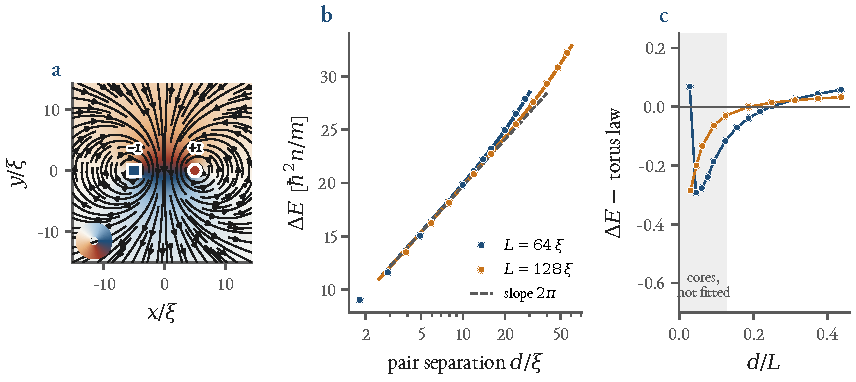
\includegraphics[width=\linewidth]{figures/ch06_coulomb.pdf}
\caption[The logarithmic interaction of vortices in the solver]{The logarithmic interaction of vortices in the solver. \textbf{a}~A vortex--antivortex pair (red disc: $+1$, blue square: $-1$), separation $d=10\,\xi$, imprinted into a
uniform condensate by \texttt{qf-pgpe} ($L=64\,\xi$); colour: phase of the field (the wheel at lower left), lines: streamlines of the superfluid velocity. \textbf{b}~Excess energy of
the imprinted pair against the separation, for $L=64\,\xi$ (blue) and $L=128\,\xi$ (orange); solid lines: the torus point-vortex law~\eqref{ch06:eq-torus} with one fitted
constant per box; dashed: the plane law with slope $2\pi$. \textbf{c}~Residual of the torus law; the shaded band is the core region $d<8\,\xi$ that was not fitted.
Source: \texttt{figures/ch06\_loglaw.py}, \texttt{ch06\_coulomb.py}.}\label{ch06:fig-coulomb}\end{figure}

For $d$ between $\cnDloSixtyfour$ and $\cnDhiSixtyfour$ $\xi$ ($\Delta E$ from $\cnElowSixtyfour$ to $\cnEhighSixtyfour$ in units $\hbar^2n/m$) in the box $L=64\,\xi$, and between
$\cnDloHundred$ and $\cnDhiHundred$ $\xi$ ($\Delta E$ from $\cnElowHundred$ to $\cnEhighHundred$) in $L=128\,\xi$, the engine follows~\eqref{ch06:eq-torus} with a single constant per
box to a root-mean-square deviation of $\cnRmsSixtyfour$ and $\cnRmsHundred$ (largest deviations $\cnMaxSixtyfour$ and $\cnMaxHundred$): about half a per cent of the
range of the energy in the root-mean-square, and less than one per cent at worst. The coefficient of the logarithm is tested more sharply by the constants: doubling the box changes $C_L$ by $2\pi\ln2=\cnTwoPiLnTwo$ if the coupling is
$2\pi\hbar^2n/m$, and the fitted constants differ by $\cnCdiff$ (the fit windows $d\ge4$, $6$, $8\,\xi$ give $\cnCdiffA$, $\cnCdiffB$, $\cnCdiff$). The naive slope of $\Delta E$ against $\ln d$ over the window $d=4$ to $8\,\xi$ is $\cnSlopeSixtyfour$ (box $64$) and
$\cnSlopeHundred$ (box $128$) times $2\pi$: the plane law is a good first guess, but the cores and the torus put a few per cent on it, and the comparison with the torus law is the
meaningful one. The Coulomb-gas coupling of the programme's projected field is therefore $2\pi\hbar^2n_s/m$ with $n_s=n$ at zero temperature, to within $0.3\%$ in the constants for every window tried, and
every instrument built on the point-vortex picture (the matching of \cref{ch06:field}, the pair statistics of \cref{ch07}) starts from a law that the engine itself obeys. The
imprint is not the relaxed vortex, so the constants themselves carry a core-mismatch energy; no claim is made about $E_c$.

\section{The flow, integrated by CVODE}\label{ch06:cvode}

\begin{rustbox}{CVODE on the Kosterlitz flow}
The flow~\eqref{ch06:eq-flow-u} is handed to CVODE through the Python module \texttt{rusty\_sundials}. Its \lstinline[style=py]{solve} returns only the end state, so a trajectory is
a chain of solves, each restarting the integrator from the previous end point (the drift reported below therefore includes the restarts). The excerpt is
verbatim from \texttt{figures/ch06\_flow\_compute.py} (\lstinline[style=py]{A_COEF} is $4\pi^3$; \lstinline[style=py]{H} is the invariant of \lean{KTFlow.kt\_invariant}; the last part is the body of the loop of the function
\lstinline[style=py]{chain}, one link of the chain per pass).
\begin{lstlisting}[style=py]
def f(u): return 2 * u - pi * math.log(u)
def H(u, y): return f(u) - 2 * pi ** 3 * y * y

def make_rhs(a=A_COEF):
    def rhs(l, s):
        u, y = s
        return [a * y * y, (2 - pi / u) * y]
    return rhs

def solver(method, rtol, atol=1e-13):
    return CvodeSolver(method=method, rtol=rtol, atol=atol, max_steps=500000)

    while l < lmax - 1e-12:
        step = dl
        if adaptive:
            step = min(dl, 0.05 / max(1.0, abs(rhs(l, s)[0])))
        l1 = min(l + step, lmax)
        try:
            _, s = sv.solve(rhs, l, s, l1)
        except RuntimeError:
            status = "solver_stop"; break
        l = l1
        L.append(l); U.append(s[0]); Y.append(s[1])
        if s[0] > ustop or abs(s[1]) > ystop:
            status = "left"; break
\end{lstlisting}
The module used for every number of this section is the build of rusty-SUNDIALS commit \cnCommitShort{} (\texttt{sha256} \cnShaShort{}\ldots, recorded in \texttt{figures/ch06\_numbers.json}). The script
refuses to run with any other: it first integrates $y'=-y$ on $[0,10]$ with Adams at $\mathrm{rtol}=10^{-8}$ and stops unless that needs fewer than $5000$ right-hand-side calls
($\cnPoneNew$ here). The printed record of the run (\texttt{figures/ch06\_flow\_compute.log}), last lines:
\begin{lstlisting}[style=plainmono]
adams_0.0001 2.2990858496996225e-05 0.020871856137751443 0.0
adams_1e-06 1.1391289778117653e-07 0.020866424221486657 0.1
adams_1e-08 2.703142154558691e-09 0.020866528666865003 0.3
adams_1e-10 1.9197976541818207e-11 0.02086653416968831 0.1
bdf_0.0001 6.019662951661786e-06 0.020866911425781565 0.2
bdf_1e-06 2.1762584490048198e-07 0.020866208945461207 0.8
bdf_1e-08 1.7298834809054142e-08 0.020866528311566324 1.0
bdf_1e-10 6.256666296167168e-10 0.020866533765439677 1.3
control [0.013523778528752306, 0.004224805752023997, 0.0009541671101744864, 0.011222398376601106, 0.2505532326600892, 0.01841533553023922]
\end{lstlisting}
(columns: method and \texttt{rtol}; the largest drift of $H$ over six trajectories to $l=40$; the smallest distance of those trajectories from $u=\pi/2$; the seconds of the run on the shared machine. Last
line: the drift of the same six trajectories of a flow whose coefficient $4\pi^3$ was changed by $5\%$ in $\dd u/\dd l$ only, the negative control.)
\end{rustbox}

\paragraph{A first-order integrator hiding in plain sight.} Our first attempt used the \texttt{rusty\_sundials} module that sits in the programme's virtual environment, and it was
slow in a way that smelled wrong: one link of $0.25$ units of $l$ cost $\cnPthreeOld$ evaluations of the right-hand side, and $20$ units cost $\cnPfourOld$. We counted. For a smooth,
slowly varying flow at $\mathrm{rtol}=10^{-9}$, a variable-order Adams method should need a few hundred. The module built from commit \cnCommitShort{} needs $\cnPthreeNew$ and
$\cnPfourNew$; on $y'=-y$ over $[0,10]$ at $\mathrm{rtol}=10^{-8}$ the old module needs $\cnPoneOld$ and the new one $\cnPoneNew$, and the old one's error is $\cnPoneOldErr$ against $\cnPoneNewErr$
(figures/ch06\_cvode\_probe.py, \texttt{ch06\_cvode\_probe\_venv.json} and \texttt{\_5db8041.json}). The old module had been built before a repair to the library: its
Adams method never left order one (it was implicit Euler with a Milne-style error estimate), and a first-order method under local error control has a global error that falls only like
the square root of the tolerance (\texttt{docs/CVODE\_ADAMS\_FIX.md} of rusty-SUNDIALS). Its answers are far less accurate than the tolerance that was asked for, and each costs a thousand times
more work; nothing in its output says so, and a user who does not count calls would not know. Our first full run with it had not finished the first of its six parts after ten minutes of
wall-clock time on the shared machine when we stopped it to count. The lesson is the programme's usual one: a solver result needs a cost figure next to it, and the script an environment check.

\paragraph{The portrait.} \Cref{ch06:fig-portrait}a shows $\cnNtraj$ trajectories integrated with Adams at $\mathrm{rtol}=10^{-9}$, drawn over the level sets of the exact invariant. Of
the $\cnNtraj$ starting points, $\cnNhyp$ satisfy the hypothesis of the trapping theorem ($u_0<\pi/2$, $H_0>f(\pi/2)$). All $\cnNhyp$ stay below $u=\pi/2$ for the whole run to $l=60$, $u$ is
monotone along each, and $y^2\le y_0^2$ throughout, as \Lthm{KTFlow}{kt_trapped}, \Lthm{KTFlow}{u_monotone} and \Lthm{KTFlow}{kt_fugacity_bounded} require; their end points lie on the line of fixed points at
the root $u_*$ of $f(u_*)=H_0$, as the invariant says they must: to $\cnUstarErrTypical$ or better for all but three of them, which start within $4\times10^{-3}$ of the separatrix in $H$ and have not
converged at $l=60$ (the worst differs from the root by $\cnMaxUstarErr$). The $\cnNbelow$ starting points on the superfluid side \emph{below} the separatrix all cross $u=\pi/2$ ($\cnNbelow$ of
$\cnNbelow$), as the new escape theorems require. And $\cnNbetween$ starting points lie between the exact separatrix and the textbook straight line $y=(\pi/2-u)/\pi^2$: the linearised
picture sends them to the disordered phase; the exact invariant, the theorem and CVODE all keep them on the superfluid side ($\cnNbetweenTrapped$ of $\cnNbetween$ trapped).

\begin{figure}[tbp]\centering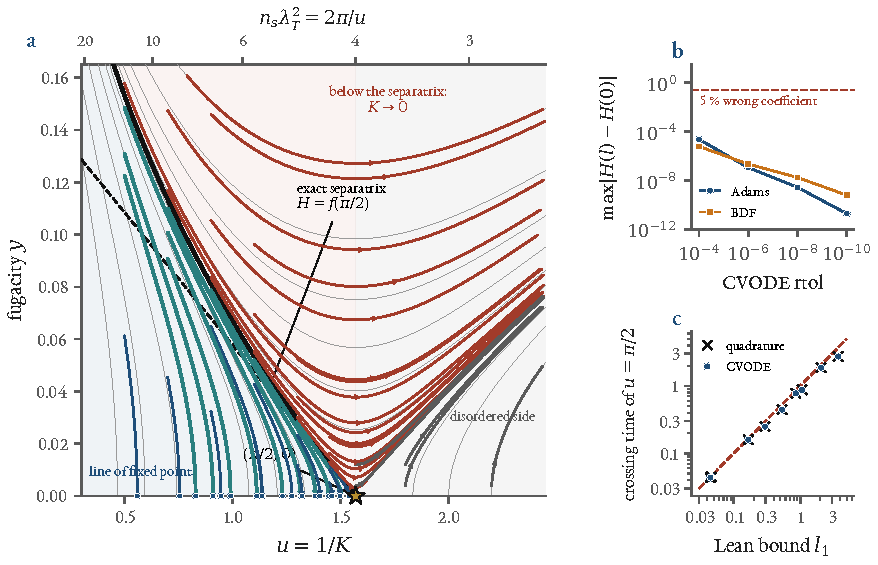
\includegraphics[width=\linewidth]{figures/ch06_portrait.pdf}
\caption[The Kosterlitz flow, integrated with CVODE]{The Kosterlitz flow, integrated with CVODE (rusty-SUNDIALS). \textbf{a}~Trajectories in the plane $(u=1/K,y)$ over the level sets of the exact invariant $H$ (thin grey lines;
by \Lthm{KTFlow}{kt_invariant} they are the flow lines). Blue: starting points that satisfy the hypothesis of \Lthm{KTFlow}{kt_trapped}; teal: those that lie between the exact separatrix
(black) and the textbook line (dashed); red: below the separatrix; grey: starting beyond $u=\pi/2$. Dots on the axis: the roots $u_*$ of $f(u_*)=H_0$. Star: the fixed point
$(\pi/2,0)$, $K=2/\pi$; the upper axis gives $n_s\lambda_T^2=2\pi/u$. \textbf{b}~Largest drift of $H$ over six trajectories ($l\le40$) against the CVODE tolerance for Adams and BDF, and for a flow with
a $5\%$ wrong coefficient (dashed red). \textbf{c}~Crossing time of $u=\pi/2$ below the separatrix, CVODE (dots) and the exact quadrature of the scalar equation (crosses), against the bound $l_1$
of \lean{kt\_escape\_time} (dashed: equality). Source: \texttt{figures/ch06\_flow\_compute.py}, \texttt{ch06\_portrait.py}.}\label{ch06:fig-portrait}\end{figure}

\paragraph{The invariant as a test of the integrator.} The theorem says $H$ is constant; the numerical $H$ is therefore a direct measurement of the global error of the integrator, with no
reference solution needed. \Cref{ch06:fig-portrait}b: with Adams the largest drift over six trajectories falls from $\cnDriftAdamsA$ at $\mathrm{rtol}=10^{-4}$ to $\cnDriftAdamsD$ at $10^{-10}$,
about as fast as the tolerance; with BDF from $\cnDriftBdfA$ to $\cnDriftBdfD$, slower at tight tolerance. The negative control shows the test has teeth: with the coefficient of $\dd u/\dd l$ wrong by $5\%$ the same
six trajectories drift by $\cnCtlLo$ to $\cnCtlHi$, that is, by $\cnCtlRatioLo$ to $\cnCtlRatioHi$ times the drift of the correct flow at the tightest tolerance. (The drift measured here includes the restart at every link; a
single call to a long interval does better, and we report the drift that a user of this interface gets.)

\paragraph{The escape bound.} For nine starting points below the separatrix (\cref{ch06:fig-portrait}c) we measure the first-passage time of $u$ through $\pi/2$ by root-finding on single CVODE solves,
and compare it with two things: the exact value of the quadrature $\int_{u_0}^{\pi/2}\dd u/(2(f(u)-H_0))$, which the scalar reduction \lean{kt\_scalar} makes available, and the Lean bound $l_1$.
CVODE and the quadrature agree to $\cnEscRelErr$ (relative), and the crossing time is below the bound in all $\cnEscN$ cases, at $\cnEscRatioLo$ to $\cnEscRatioHi$ of it. The bound uses the
smallest slope of $u$ on the way, $2(f(\pi/2)-H_0)$, which is attained only at $u=\pi/2$, so it is tight when the start is far below the separatrix and the slope is nearly the same all the way
(ratios near $1$ for the largest $f(\pi/2)-H_0$), and loose near the separatrix. This is one of the places where the proof assistant and the solver check each other: the theorem is quantitative,
and the solver tests the number.

\begin{figure}[tbp]\centering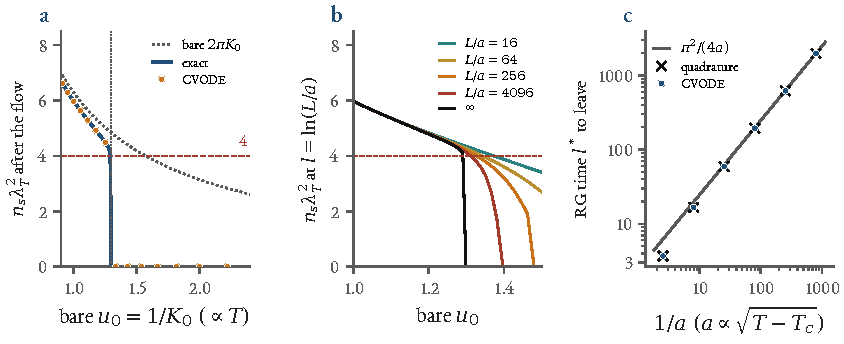
\includegraphics[width=\linewidth]{figures/ch06_jump.pdf}
\caption[The universal jump, the finite box and the essential singularity]{The universal jump, the finite box and the essential singularity in the flow (CVODE, Adams). \textbf{a}~Renormalised $n_s\lambda_T^2=2\pi K_R$ against the bare $u_0=1/K_0$ at fixed
$y_0=0.03$ (a toy: the bare fugacity is not tied to the temperature): the root of $f(u_*)=H_0$ (blue) and the end of a CVODE chain to $l=80$ (orange dots). The renormalised stiffness stays
above $4$ on the superfluid side and is $0$ beyond $u_{0c}$; the dotted curve is the bare $2\pi K_0$. \textbf{b}~The same flow stopped at $l=\ln(L/a)$, for four box sizes, and the limit $L\to\infty$:
the jump is rounded, and the crossing of the level $4$ moves to larger $u_0$ (higher temperature) in a smaller box. \textbf{c}~The scale $l^*$ at which a flow just above the separatrix leaves the critical
region, against $1/a$ with $a^2=(\pi/2)(f(\pi/2)-H_0)$, $a\propto\sqrt{T-T_c}$: CVODE (dots), quadrature (crosses), and the asymptote $\pi^2/(4a)$ (line): $\xi=e^{l^*}\sim e^{\pi^2/4a}$, the essential singularity. Source:
\texttt{figures/ch06\_flow\_compute.py}, \texttt{ch06\_jump.py}.}\label{ch06:fig-jump}\end{figure}

\paragraph{The jump.} \Cref{ch06:fig-jump}a puts the two halves of the theorem together for a one-parameter family of flows at fixed $y_0=0.03$ (a toy, the bare fugacity is not tied to the
bare stiffness here; the aim is the shape). On the superfluid side the end point of the flow is the root $u_*$ of $f(u_*)=H_0$ and the renormalised stiffness is above the universal value; the
end of a CVODE chain to $l=80$ agrees with the root (for $K_0=0.8$: $K_R=\cnKRcv$ from both). Past the critical bare stiffness, $K_{0c}=\cnKzeroC$ ($u_{0c}=\cnUzeroC$), $y$ grows and $K$ falls to zero.
Just above $K_{0c}$ the renormalised stiffness is $K_R=\cnKRgrid$ ($n_s\lambda_T^2=\cnNslGrid$) at the nearest grid point, and tends to the universal value $2/\pi$ with a square-root cusp:
$f(u)\simeq f(\pi/2)+(2/\pi)(u-\pi/2)^2$ gives $K_R-2/\pi\simeq(4/\pi^2)\sqrt{\pi\epsilon/2}$ for $H_0=f(\pi/2)+\epsilon$. This continuity is the third piece of the jump, the one that the theorems do not prove. The jump itself, from $4$ to $0$, is what Bishop and Reppy tested.

\paragraph{A finite box.} A film of size $L$ cannot flow further than $l=\ln(L/a)$. \Cref{ch06:fig-jump}b stops the flow there. The jump is rounded, and the apparent transition, the crossing of
$n_s\lambda_T^2=4$, moves to a larger bare $u_0$, that is, a higher temperature: by $\cnShiftA$, $\cnShiftB$, $\cnShiftC$ and $\cnShiftD$ of $u_{0c}$ for $L/a=16$, $64$, $256$ and $4096$. The reason
is the approach to the fixed point along the separatrix. With $x=u-\pi/2<0$ the scalar equation becomes $x'=(4/\pi)x^2(1+O(x))$, so $x\simeq-\pi/(4l)$ and
\begin{equation}
  n_s\lambda_T^2(l)=\frac{2\pi}{u}\simeq4+\frac{2}{l}\qquad\text{along the critical trajectory}
  \label{ch06:eq-critical}
\end{equation}
(Exercise~2): the critical film still looks stiffer than $4$ at any finite scale, and only logarithmically so. CVODE agrees: $l\,(n_s\lambda_T^2-4)$ along the separatrix is
$\cnCritA$ at $l=10$, $\cnCritB$ at $l=10^2$ and $\cnCritC$ at $l=10^4$, tending to $2$, with the invariant conserved to $\cnCritDrift$ over the whole run.

\paragraph{Above the transition.} For a flow that starts just below the separatrix, $H_0=f(\pi/2)-\epsilon$, the scalar equation near the fixed point is $x'=(4/\pi)(x^2+a^2)$ with
$a^2=(\pi/2)\epsilon$, and the time to cross from $-X$ to $X$ is $(\pi/4a)\,2\arctan(X/a)\to\pi^2/(4a)$: the flow lingers at the fixed point for a time that diverges as $1/\sqrt{\epsilon}$, and since
$\epsilon$ is linear in the distance from the critical temperature, the correlation length $\xi\sim e^{l^*}$ diverges as $\exp(b/\sqrt{T-T_c})$. \Cref{ch06:fig-jump}c: the time for the flow to
reach $u=2$ from $u_0=0.8$, by quadrature and by CVODE, divided by $\pi^2/(4a)$ is $\cnEssRatioA$, $\cnEssRatioB$ and $\cnEssRatioC$ for $\epsilon=10^{-1}$, $10^{-3}$ and $10^{-6}$; the difference
$l^*-\pi^2/(4a)$ settles at $-\cnEssOffset$, a constant that depends on where one chooses to stop. CVODE and the quadrature differ by $\cnEssRel$ (relative) at the smallest $\epsilon$.

The flow equations are a model; everything so far says that the model is internally consistent with the theorems and that CVODE integrates it correctly. Whether a fluid obeys it is another question,
and the next section asks it of the solver's own fluid.

\section{The simulated field near the transition}\label{ch06:field}

The engine of \cref{ch06:coulomb} is a classical field: the projected Gross--Pitaevskii equation, started from a random state of chosen total energy, thermalises, and its
temperature is \emph{measured} from the trajectory (equipartition of the modes near the cutoff), not imposed. It is a weakly interacting Bose gas with a cutoff, not helium; the
Kosterlitz--Thouless mechanism needs only a stiff phase and vortices, and the field has both (this is the property the analogy with the film depends on, in the sense of the
programme's rule LL-15), but a number measured here is a number of this model. The \emph{heating ladder} of the programme's second round starts from two equilibrated cold states (energy per particle $e=0.90$, evolved to $t=4000$, two seeds), adds random phonons
until the total energy reaches the target, and raises $e$ in nine steps, $e=1.00,1.05,\dots,1.40$, in a periodic box of side $L=64\,\xi$; each run has a transient of $500$ time units and is
averaged over $t=500$ to $1500$ (\texttt{data/generated/pgpe/r2/}, files \texttt{II\_*.json}). The steps above $e=1.20$ were added after the log of the first runs showed that the crossing
lay above the range that had been pre-registered (amendment R2-A4 of the programme, written before any verdict was computed). A smaller box, $L=32\,\xi$, with five energies and three
seeds, was run to see the size dependence; those runs start from random states and last $4000$ time units, with the last $1000$ sampled, so the comparison of the two boxes inherits
a difference of protocol. For each run we recompute from the saved per-run records (\texttt{figures/ch06\_pgpe\_data.py}, which agrees with the programme's own analysis to the last digit)
\begin{itemize}
\item $T$, from equipartition of the high-wavenumber modes, in units $\hbar^2/(m\xi^2)$ with $k_B=1$;
\item $n_s/n$, from the transverse and longitudinal current correlators at the smallest wavevectors, $n_s/n=1-\langle|J_T|^2\rangle/\langle|J_L|^2\rangle$, and from it
$n_s\lambda_T^2=(n_s/n)\,2\pi/T$ (for $n=1$, $\lambda_T^2=2\pi/T$);
\item $\eta$, from a fit of $g_1(r)\sim r^{-\eta}$ over a window that excludes the noise floor;
\item the vortices, by the winding rule of \lean{VortexWinding} (the sum of the principal-value phase differences around a plaquette is an exact multiple of $2\pi$).
\end{itemize}
Only runs that pass the programme's equilibrium admission test (the longitudinal and transverse current fluctuations must not exceed what an equilibrium state allows) enter; all 18
runs of the $L=64$ ladder and all 15 of the $L=32$ series pass. \Cref{ch06:tab-ladder} gives the seed means.

\begin{table}[t]\centering\small
\caption{The heating ladder, $L=64\,\xi$: seed means of $T$, superfluid fraction, $n_s\lambda_T^2$, the exponent $\eta$ of $g_1$, the product $\eta\,n_s\lambda_T^2$ (equal to $1$ for a
Gaussian phase field, \cref{ch06:eq-eta}), and the number of vortices (all runs, both signs). Source: \texttt{figures/ch06\_pgpe\_numbers.json}.}\label{ch06:tab-ladder}
\begin{tabular}{@{}rrrrrrr@{}}\toprule
$e$ & $T$ & $n_s/n$ & $n_s\lambda_T^2$ & $\eta$ & $\eta\,n_s\lambda_T^2$ & $N_v$\\\midrule
% BEGIN ch06 table
1.00 & 0.571 & 0.809 & 8.90 & 0.126 & 1.12 & 19\\
1.05 & 0.622 & 0.767 & 7.75 & 0.145 & 1.12 & 32\\
1.10 & 0.668 & 0.725 & 6.82 & 0.164 & 1.12 & 47\\
1.15 & 0.722 & 0.703 & 6.11 & 0.192 & 1.18 & 66\\
1.20 & 0.775 & 0.647 & 5.24 & 0.230 & 1.20 & 90\\
1.25 & 0.818 & 0.533 & 4.09 & 0.297 & 1.22 & 117\\
1.30 & 0.862 & 0.370 & 2.70 & 0.447 & 1.21 & 147\\
1.35 & 0.906 & 0.357 & 2.48 & 0.540 & 1.34 & 179\\
1.40 & 0.966 & 0.255 & 1.66 & 0.660 & 1.09 & 212\\
% END ch06 table
\bottomrule\end{tabular}\end{table}

\Cref{ch06:fig-field}d shows the stiffness. It falls through the Nelson--Kosterlitz level $n_s\lambda_T^2=4$ between $e=1.25$ and $e=1.30$; interpolating the seed means, the crossing
is at $T_{\rm BKT}(L{=}64)=\cnTbktSixtyfour$, where $\eta=\cnEtaCrossSixtyfour$ (the infinite-size value is $1/4$) and $n_s/n=\cnNsOverNCross$. The two seeds do not agree on where the
crossing is: taken separately they give $\cnTbktSeedLo$ and $\cnTbktSeedHi$; this is the honest error bar of the number. At $e=1.25$ the two seeds read $n_s\lambda_T^2=\cnKseedA$ and
$\cnKseedB$, on either side of $4$. In the smaller box the crossing is at $T_{\rm BKT}(L{=}32)=\cnTbktThirtytwo$ (seeds: $\cnTbktSeedLoThirtytwo$ to $\cnTbktSeedHiThirtytwo$, which does not overlap the
range of the larger box), and the fall of the stiffness is gentler: the slope $|\dd(n_s\lambda_T^2)/\dd T|$ at the crossing is $\cnSlopeCrossSixtyfour$ for $L=64$ and $\cnSlopeCrossThirtytwo$ for
$L=32$. Both signs, a crossing at a higher temperature and a softer fall in the smaller box, are what the flow predicts when it is stopped at the scale of the box: a film of size
$L$ sees the stiffness $K(l)$ at $l=\ln(L/a)$, and along the critical trajectory this exceeds $2/\pi$ by an amount that shrinks only as $1/l$ (\cref{ch06:fig-jump}b and
Exercise~2). The toy flow of that figure has two parameters that we did not fit to the field, and the agreement is one of sign and not of number: between $L/a=32$ and $64$ the toy moves the crossing, in temperature, by $\cnShiftToy\%$, and the field
between $L=32\,\xi$ and $64\,\xi$ by $\cnShiftField\%$.

\begin{figure}[t]\centering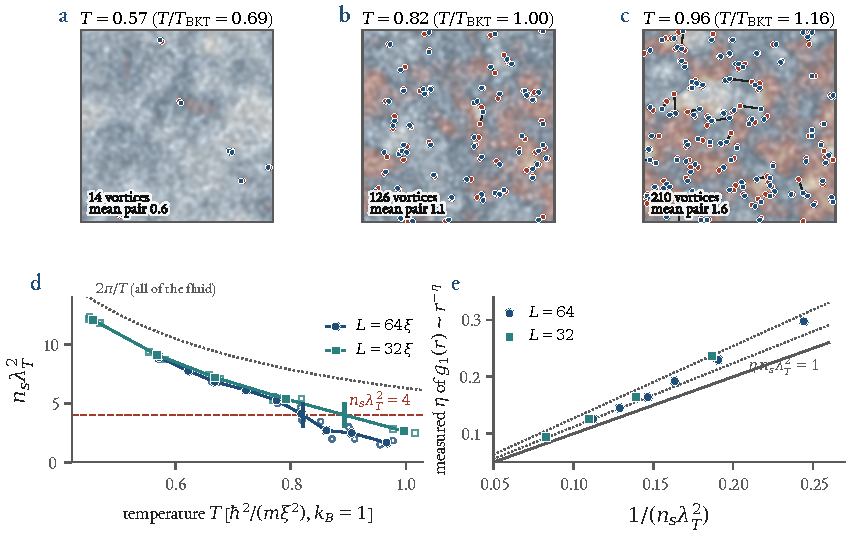
\includegraphics[width=\linewidth]{figures/ch06_field.pdf}
\caption[The simulated Bose field near the transition]{The simulated Bose field near the transition. \textbf{a--c}~Final states of the $L=64\,\xi$ heating ladder at $T=0.57$, $0.82$ and $0.96$ (in units of
$T_{\rm BKT}(64)=0.82$: $0.69$, $1.00$, $1.16$): vortices ($+1$ red, $-1$ blue) found by the winding rule, the optimal pairing of positive to negative vortices as black bonds, and
the coarse-grained phase as background hue; positions are on the grid, so separations below $0.5\,\xi$ are not resolved. \textbf{d}~$n_s\lambda_T^2$ against $T$: single runs (open
symbols) and seed means (filled) for $L=64$ (blue) and $L=32$ (teal); the red dashed line is the universal level $4$, the ticks mark the interpolated crossings, the dotted line is
$2\pi/T$, the value if the whole fluid were superfluid. \textbf{e}~Measured $\eta$ against $1/(n_s\lambda_T^2)$ for the energies with $n_s\lambda_T^2>4$; the grey line is the
spin-wave relation $\eta\,n_s\lambda_T^2=1$, the dotted lines are $12$ and $27\%$ above it. Source: \texttt{figures/ch06\_field.py}.}\label{ch06:fig-field}\end{figure}

\paragraph{What does not come out as the theory says.} Three things. First, the classical field at the crossing has $n\lambda_T^2=2\pi/T_{\rm BKT}=\cnNlambda$, against
$\ln(380/\tilde g)=\cnLnThreeEighty$ for the weakly interacting gas without a cutoff (Prokof'ev, Ruebenacker and Svistunov~\cite{Prokofev2001}; $\tilde g=1$ here, which is not small):
$\cnNlambdaExcess\,\%$ more. The programme's literature review suggested that this is the ultraviolet logarithm of a classical field with a sharp cutoff; the estimate it gives for our cutoff,
$T_{\rm BKT}=0.811$ and $n\lambda_T^2=7.75$, is close to the measured values, but that was a hypothesis when this chapter was written, not a test, and we do not use it. Second, the
spin-wave relation. For the six energies with $n_s\lambda_T^2>4$ the product $\eta\,n_s\lambda_T^2$ is $\cnEtaKlo$ to $\cnEtaKhi$ (\cref{ch06:fig-field}e), and for $L=32$ it is
$\cnEtaKloThirtytwo$ to $\cnEtaKhiThirtytwo$: a systematic excess of $12$ to $27\%$ over $1$, which is outside the scatter of the seeds. The programme's larger boxes ($L=128$ and $192$) show an
excess that is also positive at every size and not monotone in $L$; its origin is unknown to us, and \cref{ch10} lists it among the open items. Third, the round-1 value
$T_{\rm BKT}\approx0.72$, interpolated between states that were started by a quench, is withdrawn: those states were not equilibrated (at the same vortex count they had half the
stiffness of the heated ones), and $0.821$ replaces it.

\paragraph{Vortex positions against the two Lean statements.} \Cref{ch06:fig-field}a--c show what the optimal pairing looks like. At the lowest temperature almost all vortices are
in tight pairs (the mean matched separation is $\cnPairLo\,\xi$, at the resolution of the grid); at $T_{\rm BKT}$ there are $\cnNvMid$ vortices in the box with a mean matched
separation of $\cnPairMid\,\xi$; at $T=0.96$ the pairs are $\cnPairHi\,\xi$ long and the bonds begin to reach across the box. We now apply the two statements of \cref{ch06:lean} to
every configuration at hand: the final fields of the two series ($33$ configurations) and the saved positions of six $L=192$ runs ($100$ snapshots each, $t=13\,510$ to $14\,500$, the last window of the programme's longest runs; five of the six are equilibrated, the sixth, $e=1.10$ seed $11$, still carries one pair
of the size of the box). For each configuration we find the optimal matching $W$ with minimum-image distances, and evaluate $|\rho(k)|/|k|$ on the
reciprocal lattice (all $|n_x|,|n_y|\le6$).

\begin{figure}[t]\centering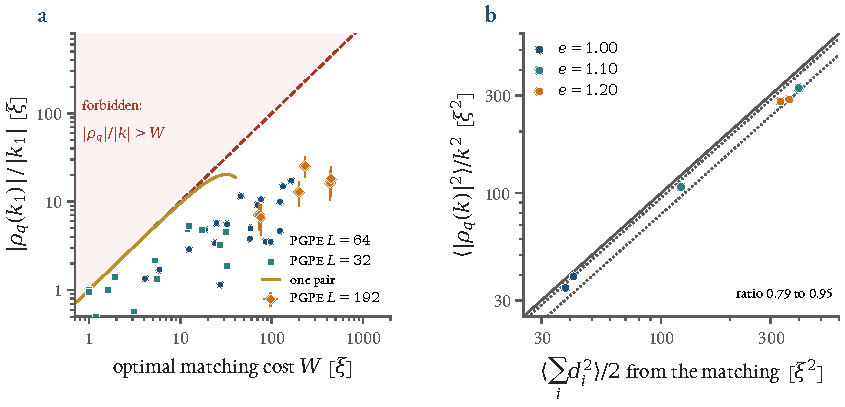
\includegraphics[width=\linewidth]{figures/ch06_screening.pdf}
\caption[The two Lean statements about vortex positions, tested on the solver's configurations]{The two Lean statements about vortex positions, tested on the solver's configurations. \textbf{a}~$|\rho_q(k_1)|/|k_1|$ at the smallest wavevector against the optimal
matching cost $W$: $33$ final fields of the $L=64$ and $L=32$ series (symbols), the six $L=192$ runs (mean and standard deviation over $100$ snapshots), and one isolated pair of
separation $d$ in a box of $64\,\xi$ (gold curve). The red dashed line is the bound of \Lthm{MatchingScreening}{norm_rho_le_matching_torus}: no point may lie above it, and none does. \textbf{b}~The polarisability
plateau $\langle|\rho_q(k)|^2\rangle/k^2$ (mean over the shells $m^2=4,\dots,16$) against $\langle\sum_id_i^2\rangle/2$ from the optimal matching, for the six $L=192$ runs; the dotted
lines are $0.79$ and $0.95$ times the diagonal. Source: \texttt{figures/ch06\_certificates.py}, \texttt{ch06\_screening.py}.}\label{ch06:fig-screening}\end{figure}

\emph{The matching bound.} There is no violation in any of the $\cnNconfigs$ configurations, nor in any of the $600$ snapshots of the $L=192$ runs, on any of the wavevectors tried.
That the inequality holds is no surprise, since it is a theorem; what the data show is how much room it leaves. For a thermal gas of tight pairs the bound is loose: the ratio
$\tau=|\rho(k_1)|/(|k_1|W)$ is $\cnTauLoFields$ to $\cnTauHiFields$ for the fields (the large values are the configurations with one or two pairs) and $\cnTauLoRuns$ to $\cnTauHiRuns$ for the
$L=192$ runs, because the pairs cancel each other's charge at a long wavelength while the matching cost counts every one of them. The bound is saturated only by an isolated pair
whose separation is small against the wavelength, $\tau=\sin(k_1d/2)/(k_1d/2)\to1$ (Exercise~3). It is a certificate, not a detector: it bounds the total pairing length from below
whatever the configuration (a charge density of order one at the smallest wavevector requires the vortices of opposite sign to be, in total, at least $L/2\pi$ apart), and a small value
certifies nothing.

\emph{The polarisation form.} At the four shortest wavevectors the premise $|k\cdot d_i|\le1$ of \Lthm{PairPolarisation}{rho_polarisation} holds for every pair in $\cnPremiseOk$ of the $\cnNconfigs$ field
configurations, and in all of them the inequality $|\rho-i\sum_i(k\cdot d_i)e^{ik\cdot m_i}|\le\sum_i(k\cdot d_i)^2$ holds, with the pairs taken from the optimal matching. The typical size of the remainder
is $\cnRemMed$ of $|\rho|$ (median), and the bound on it is $\cnBoundMed$ of $|\rho|$: in a thermal gas of pairs the long-wavelength vortex charge density is, to about
$\cnRemMedPct\,\%$ (median over the configurations), the divergence of a polarisation density. That is the dielectric picture in numbers. Its consequence for the stiffness is Kosterlitz and Thouless's $\varepsilon-1\propto\sum d^2$,
and \cref{ch06:fig-screening}b checks it on the six $L=192$ runs: the long-wavelength charge fluctuations per $k^2$ are $\cnDfourLo$ to
$\cnDfourHi$ of the sum of $d_i^2/2$ over the matched pairs, always below it; the programme reads the deficit as the screening of dipoles by dipoles, which we did not test separately. We re-derived these numbers with independent code, because the file stored in the repository
for them (\texttt{data/generated/pgpe/dielectric/primary\_C4.json}) still holds the values from before a correction, about $0.009$ (a factor $k^2$ applied by mistake, as
\texttt{PGPE\_DIELECTRIC\_RESULTS.md} records); our values match the corrected table of that document. What the dielectric analysis does \emph{not} give is a mode-by-mode relation between the
transverse current and the detected charges: the pre-registered test of that failed in five of six runs, the coherence being $0.06$ to $0.28$.

\section{What this chapter establishes, and what it does not}\label{ch06:honest}

\begin{honestbox}
\textbf{Proved in Lean} (kernel-checked; every declaration depends only on \texttt{propext}, \texttt{Classical.choice}, \texttt{Quot.sound}). In the library: the exact invariant and the trapping
of the Kosterlitz flow, the monotonicity of $u$, the bound on the fugacity and the unit conversion ($K>2/\pi\iff n_s\lambda_T^2>4$) \emph{for solutions defined for every real $l$}; the bound of
the vortex charge density by every pairing of the vortices (plane and torus); the polarisation form of the charge density of pairs. In the new module of this book
(\texttt{book/lean/Ch06\_KTForward.lean}, $18$ declarations audited, no \lstinline[style=lean]{sorry}): the same statements for solutions on $l\ge0$ only, the escape bound and escape time below the separatrix,
the vanishing of $K$ there, the dichotomy at the separatrix, and the theorem that the library's hypotheses leave only fixed points on the superfluid side. \emph{Not} formalised: that non-trivial
solutions on $[0,\infty)$ exist; that $K_R\to2/\pi$ as the invariant tends to $f(\pi/2)$ from above; the flow equations themselves, which are Kosterlitz's leading-order equations, taken as given.

\textbf{Computed} (CVODE from rusty-SUNDIALS commit \cnCommitShort{}; \texttt{qf-pgpe} as installed on the machine, its build commit not recorded; one shared, loaded machine). CVODE integrates the flow with the invariant conserved to $\cnDriftAdamsD$ (Adams, $\mathrm{rtol}=10^{-10}$, chain of
solves), reproduces the exact first-passage times to $\cnEscRelErr$ and keeps all $\cnNhyp$ trapped starting points trapped; the engine \texttt{qf-pgpe} follows the torus point-vortex law for the energy of an imprinted
pair to a root-mean-square deviation of $\cnRmsSixtyfour$ ($L=64$) and $\cnRmsHundred$ ($L=128$) in units of $\hbar^2n/m$, and the coefficient $2\pi\hbar^2n/m$ of the logarithm to $0.3\%$. The classical field has an
$n_s\lambda_T^2$ that crosses $4$ at $T_{\rm BKT}(64)=\cnTbktSixtyfour$ (seeds $\cnTbktSeedLo$ to $\cnTbktSeedHi$) and $T_{\rm BKT}(32)=\cnTbktThirtytwo$; these come from runs of the programme's numpy engine
(two seeds for $L=64$, three for $L=32$), recomputed here from the raw records, not re-run. The two Lean statements about vortex positions were tested on $\cnNconfigs$ configurations and $600$ snapshots and are
never violated.

\textbf{Measured.} The only experiment of this chapter is Bishop and Reppy's, as its abstract reports it: no film data were analysed, and nothing here is a statement about helium except that jump formula and the
number $\cnJump\times10^{-9}\ \mathrm{g\,cm^{-2}\,K^{-1}}$ computed from it. The simulated field is a classical Bose gas with a cutoff, in units where $\tilde g=1$ is not small; the match with a film is the
shared mechanism (a stiff phase with vortices), not a quantitative identity. The Godfrin measurements are of a different system (a Fermi liquid) and enter only through the dimension.

\textbf{Analogy, not result.} The toy flow of \cref{ch06:fig-jump} gives the sign of the finite-size shift of the transition but about one per cent where the field shows nine; its bare parameters were not fitted.

\textbf{Failed, withdrawn or open.} (i)~The round-1 transition temperature $T_{\rm BKT}\approx0.72$ of the programme, from quench-started states, is withdrawn in favour of $0.821$ (the quench states were not equilibrated).
(ii)~The spin-wave relation $\eta\,n_s\lambda_T^2=1$ is violated by a systematic $12$--$27\%$ at $L=32$ and $64$, and by a positive and non-monotone amount at larger sizes; unexplained. (iii)~The programme's
pre-registered mode-by-mode relation between the transverse current and the detected vortex charges failed (five of six runs); only the polarisability plateau holds (ratios $\cnDfourLo$ to $\cnDfourHi$).
(iv)~$n\lambda_T^2$ at the crossing is $\cnNlambdaExcess\%$ above the weak-coupling value $\ln380$; the cutoff explanation was not tested. (v)~Seeds: two (or three) per point; the transition temperature is known to $\pm0.014$ ($L=64$)
at best. (vi)~\emph{Found while writing this chapter}: the hypotheses of the library theorems \lean{KTFlow} cover only fixed points on the superfluid side (the library file is unchanged; the repaired statements
live in the book's module); the Python CVODE module of the project's environment predates the Adams repair and costs a thousand times more per result, and the current build's \lstinline[style=py]{solve} does not handle an output
time before the initial time; and the file \texttt{primary\_C4.json} stores pre-correction values of the polarisability ratio.
\end{honestbox}

\section*{Exercises}

\paragraph{Exercise 1.} Show that for $\dd u/\dd l=c\,y^2$ and $\dd y/\dd l=(2-\pi/u)\,y$, with any constant $c>0$, the function $2u-\pi\ln u-\tfrac c2\,y^2$ is conserved. Expand it
near $(\pi/2,0)$ and show that the level sets are the hyperbolas $x^2-(\pi c/4)\,y^2=\mathrm{const}$, $x=u-\pi/2$, with straight separatrices $y=\pm x/\pi^2$ for $c=4\pi^3$. What changes in the
statement of the trapping theorem if $c$ is replaced by another constant? \emph{Hint:} differentiate; $f''(\pi/2)=4/\pi$, so $f(u)\simeq f(\pi/2)+(2/\pi)x^2$.

\paragraph{Exercise 2.} Prove~\eqref{ch06:eq-critical}: along the separatrix $n_s\lambda_T^2(l)=4+2/l+o(1/l)$, and more precisely $l\,(n_s\lambda_T^2-4)=2-\tfrac23\,(\ln l)/l+O(1/l)$. \emph{Hint:} on the separatrix
$H=f(\pi/2)$ and the scalar equation gives $x'=2\big(f(\pi/2+x)-f(\pi/2)\big)=(4/\pi)x^2-(16/3\pi^2)x^3+\dots$; integrate $\dd(1/x)/\dd l=-x'/x^2$, first with the leading term
($1/x\simeq-4l/\pi$), then once more to get the logarithm; then $2\pi/u=4/(1+2x/\pi)$. Compare with the values of $l\,(n_s\lambda_T^2-4)$ quoted in \cref{ch06:cvode}: the expression
$2-\tfrac23(\ln l)/l$ differs from them by $\cnCritDevB$ at $l=100$ and by $\cnCritDevC$ at $l=10^4$.

\paragraph{Exercise 3.} For one vortex--antivortex pair of separation $d$, show that $|\rho(k)|/|k|=2\sin(kd/2)/k$ when $k\parallel d$, hence that the ratio $\tau=|\rho(k)|/(|k|\,W)$ of
\Lthm{MatchingScreening}{norm_rho_le_matching} equals $\sin(kd/2)/(kd/2)$. Evaluate it for the smallest wavevector $k_1=2\pi/L$ of a box of side $L$ and a pair of size $d=L/2$, and compare with the gold
curve of \cref{ch06:fig-screening}a. Why can $\tau$ be close to $1$ only when $kd\ll1$, and what does that say about reading a small charge structure factor as evidence for short pairs?
\emph{Hint:} $|e^{i\varphi}-1|=2|\sin(\varphi/2)|$.

\section*{Notes and further reading}

The unbinding of vortex pairs as the mechanism of the two-dimensional transition is due to Kosterlitz and Thouless~\cite{KosterlitzThouless1973}; Berezinskii analysed the low-temperature state of
two-dimensional systems with a continuous symmetry independently~\cite{Berezinskii1971}, and the absence of long-range order they build on is the theorem of Mermin and
Wagner~\cite{MerminWagner1966} and of Hohenberg~\cite{Hohenberg1967}. The flow equations are Kosterlitz's~\cite{Kosterlitz1974}, the universal jump is Nelson and Kosterlitz's~\cite{NelsonKosterlitz1977},
and the experiment on helium films is Bishop and Reppy's~\cite{BishopReppy1978}, analysed with the dynamic theory of Ambegaokar, Halperin, Nelson and Siggia~\cite{AHNS1978,AHNS1980}. Minnhagen's
review~\cite{Minnhagen1987} covers the Coulomb gas, Kosterlitz's equations and the experiments on helium films, in the language used here. The same crossover was later studied in a trapped atomic gas~\cite{Hadzibabic2006};
the critical phase-space density of the weakly interacting gas is the subject of~\cite{Prokofev2001,ProkofevSvistunov2002}; classical-field simulations of the pairing and unbinding of vortices
are those of Simula and Blakie~\cite{SimulaBlakie2006} and of Foster, Blakie and Davis~\cite{FosterBlakieDavis2010}; Hasenbusch's Monte Carlo study of the XY model at the transition~\cite{Hasenbusch2005}
derives and tests the finite-size behaviour of the helicity modulus there. For point vortices on a torus see Weiss and McWilliams~\cite{WeissMcWilliams1991}. The records of the programme behind this chapter are, in the
repository, \texttt{LEDGER.md} (CLAIM-072 for \lean{KTFlow}, CLAIM-070 and CLAIM-085 for the vortex-position statements and the dielectric analysis), \texttt{docs/designs/PGPE\_R2\_RESULTS.md} (the ladder),
\texttt{PGPE\_DIELECTRIC\_RESULTS.md} and \texttt{PGPE\_ONSAGER\_RESULTS.md}. The friction and diffusion of a single vortex in the same field are the subject of \cref{ch07}.
